\documentclass[table]{beamer}
\usepackage[utf8]{inputenc}
\usepackage[squaren]{SIunits}
\usepackage{varwidth,setspace}
\usepackage{tikz}
\usetikzlibrary{intersections,positioning,backgrounds,fit,matrix,shapes,calc,decorations.pathmorphing,decorations.text,decorations.pathreplacing}
\usetheme{default}

\newcommand*{\mimg}[2]{\begingroup
\setbox0=\hbox{\includegraphics[height=#2]{#1}}\parbox{\wd0}{\box0}\endgroup}
\newcommand*{\rmimg}[2]{\begingroup
\setbox0=\hbox{\includegraphics[angle=90,origin=c,height=#2]{#1}}\parbox{\wd0}{\box0}\endgroup}
\newcommand*{\symok}[0]{\includegraphics[height=1em]{symbol_ok.pdf}}
\newcommand*{\symbad}[0]{\includegraphics[height=1em]{symbol_bad.pdf}}
\newcommand*{\symidk}[0]{{\bf\color{blue}\Large?}}

\setbeamertemplate{navigation symbols}{}%remove navigation symbols
\setbeamertemplate{footline}{\hspace*{.5cm}\scriptsize{\hfill\raisebox{1mm}{\insertframenumber}\hspace*{.5cm}}}

\setlength{\tabcolsep}{0.5mm}

\title{ACTPOL talk}
\author{Sigurd Kirkevold Næss}
\institute{Subdepartment of astrophysics, Oxford University}
\date{February, 2015}

\begin{document}

\begin{frame}
	\titlepage
	\vspace{-1cm}
	\begin{center}
	{\footnotesize The source code for this talk can be found at {\color[rgb]{0,0.7,0}https://github.com/amaurea/actpol-talk-2015}}
	\end{center}
\end{frame}

% 45 min talk, should have time to go through how we make maps
% Reuse foreground lensing too?
%
% === Map stuff ===
% Full-sky planck cmb
% zoom on patch
% compare with actpol, looks similar due to large-mode dominance
% gradually subtract large-scale modes to reveal all the small-scale modes
% highlight non-cmb features: point sources, clusters
% illustrate white noise vs correlated noise
% actpol TOD power spectrum -> actpol noise angular power spectrum
% map distortions - flat sky, boosting, lensing
%
% === Telescopes ===
% Planck: Full-sky, multi-frequency, shallow, low-res (l<2500)
% Bicep:  Small patch, very deep, low-res
% Polarbear: Small patch, deep, ?-res
% ACT,SPT: Small-medium patches, deep, high-res (l<10000)

% === Physics ===
% What can you do with high resolution?
%  ns, Neff
%  lensing -> neutrino mass, modified gravity tests?, measure galaxy bias by cross-correlation
%   explain why high res is good for lensing
%   in the low noise limit you need more modes to beat down cosmic variance
%  sz clusters -> Tsz, Ksz. Ksz probes velocity field
%  point sources - are these useful?

% === ACTPol status and plans ===
% Analysing S2 of actpol data, preparing for S3 observing with new frequencies
% Advanced actpol

\begin{frame}
	\centering
	\begin{tabular}{c}
		\only<1>{Planck}%
		\only<2>{Planck+actpol}%
		\only<3>{Planck+actpol $\ell>2000$}%
		\only<4>{Planck $\ell>2000$}%
		\\
		\only<1>{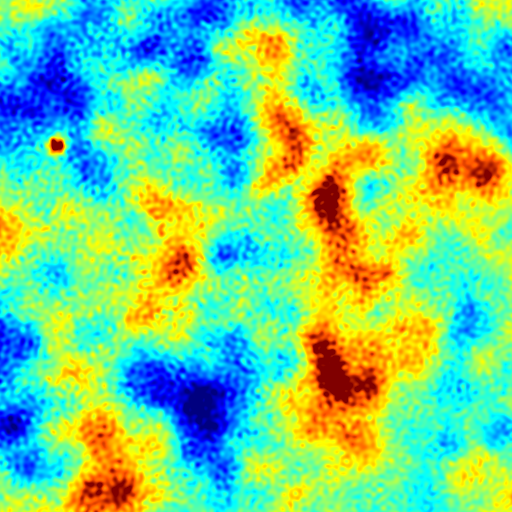
\includegraphics[width=0.7\textwidth]{maps/crop/planck.png}}%
		\only<2>{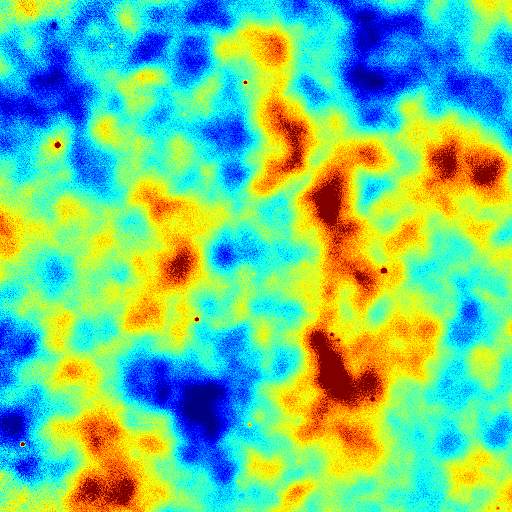
\includegraphics[width=0.7\textwidth]{maps/crop/coadd.png}}%
		\only<3>{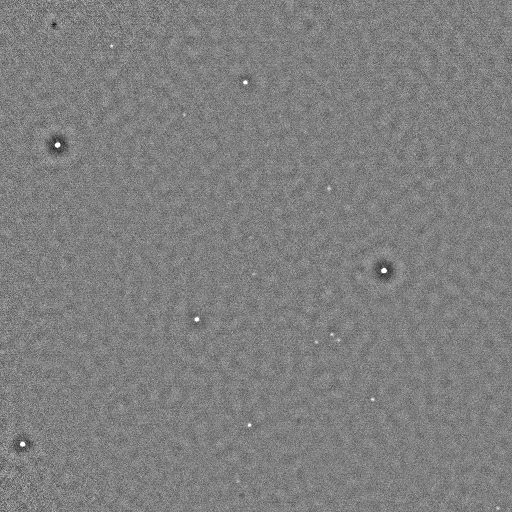
\includegraphics[width=0.7\textwidth]{maps/crop/coadd_2000_gray_0.png}}%
		\only<4>{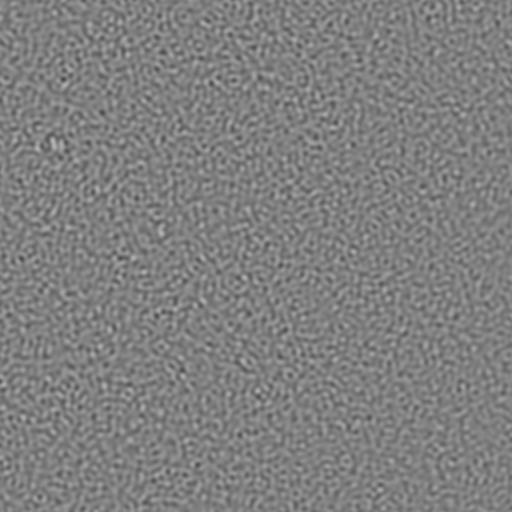
\includegraphics[width=0.7\textwidth]{maps/crop/planck_2000_gray.png}}%
		\\
		\only<1>{$\pm 250 \mu$K, $4.26^\circ \times 4.26^\circ$}%
		\only<2>{$\pm 250 \mu$K, $4.26^\circ \times 4.26^\circ$}%
		\only<3>{$\pm 200 \mu$K, $4.26^\circ \times 4.26^\circ$}%
		\only<4>{$\pm 200 \mu$K, $4.26^\circ \times 4.26^\circ$}%
	\end{tabular}
\end{frame}

\begin{frame}
	\centering
	\begin{tabular}{c}
		\only<1>{Total signal}%
		\only<2>{CMB (Wiener)}%
		\only<3>{Remainder}%
		\only<4>{Total signal}%
		\\
		\only<1>{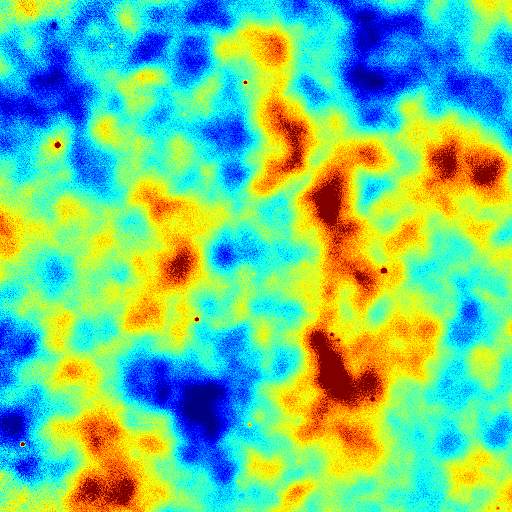
\includegraphics[width=0.7\textwidth]{maps/crop/coadd.png}}%
		\only<2>{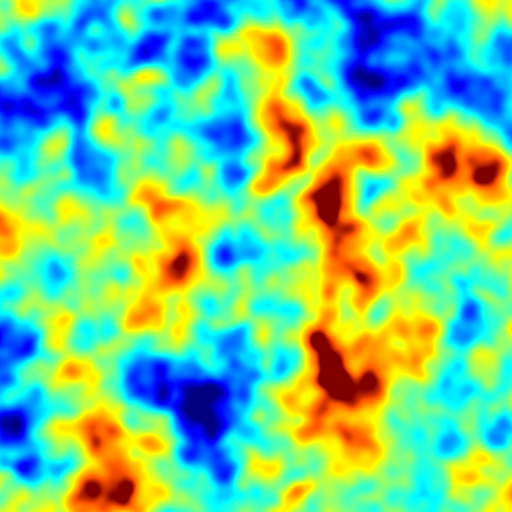
\includegraphics[width=0.7\textwidth]{maps/crop/cmb.png}}%
		\only<3>{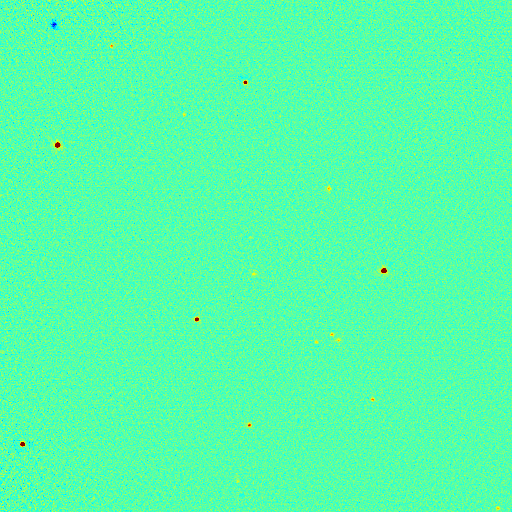
\includegraphics[width=0.7\textwidth]{maps/crop/nocmb.png}}%
		\only<4>{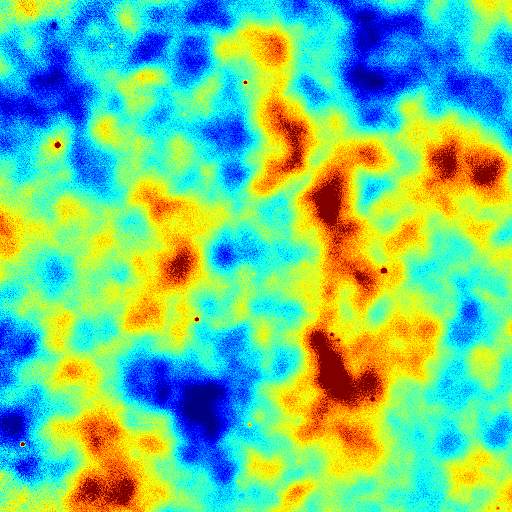
\includegraphics[width=0.7\textwidth]{maps/crop/coadd.png}}%
		\\
		$\pm 250 \mu$K, $4.26^\circ \times 4.26^\circ$
	\end{tabular}
\end{frame}

\begin{frame}{Instrument noise properties}
	\centering
	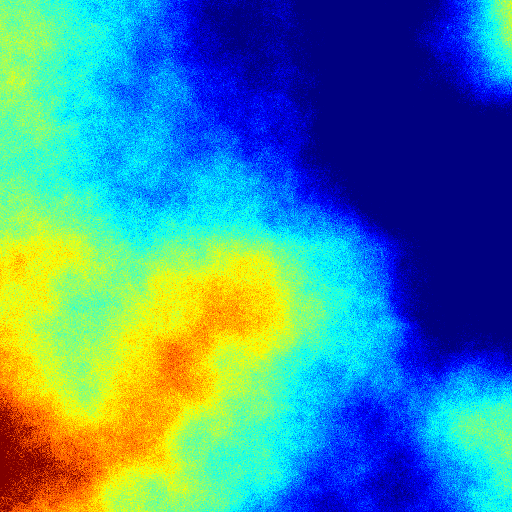
\includegraphics[width=0.7\textwidth]{maps/noise_sim.png}
\end{frame}
\begin{frame}{CMB sim for comparison}
	\centering
	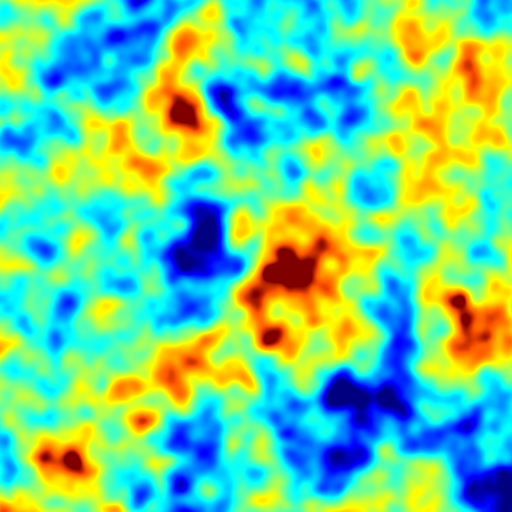
\includegraphics[width=0.7\textwidth]{maps/cmb_sim.png}
\end{frame}

\begin{frame}
	\centering
	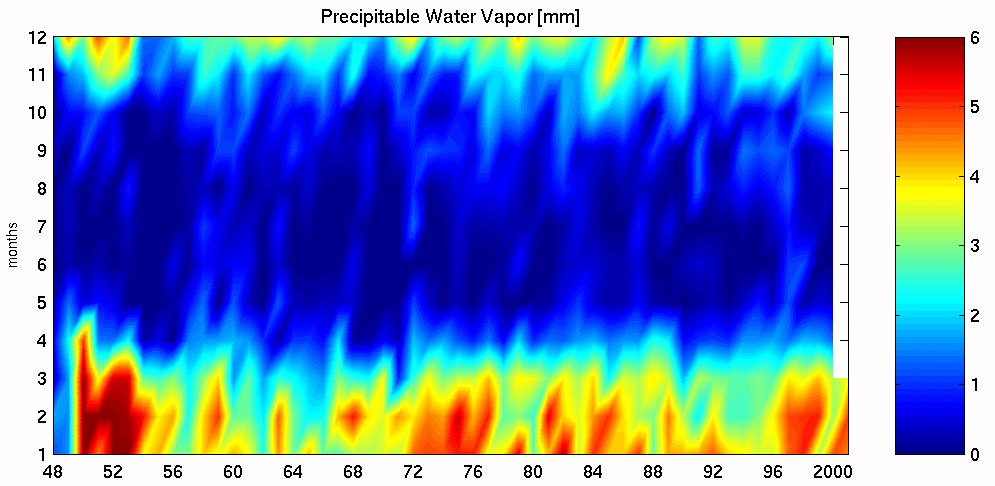
\includegraphics[width=\textwidth]{pwv_chajnantor_eso.jpeg}
\end{frame}

\begin{frame}{Lensing distorts the CMB}
	\begin{center}
		\begin{tikzpicture}
			\only<1>{\node at (0,0) {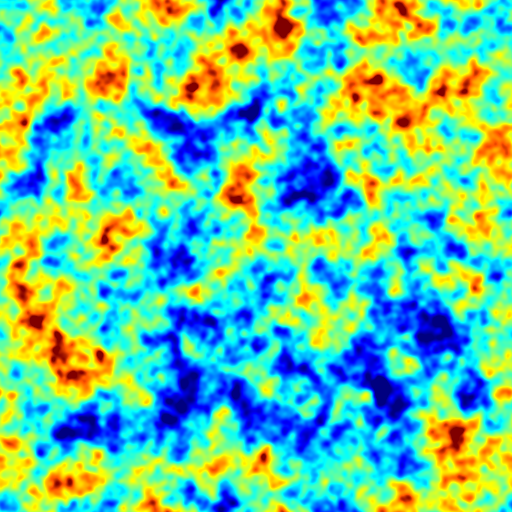
\includegraphics[height=7cm]{lensing/T.png}};}%
			\only<2>{\node at (0,0) {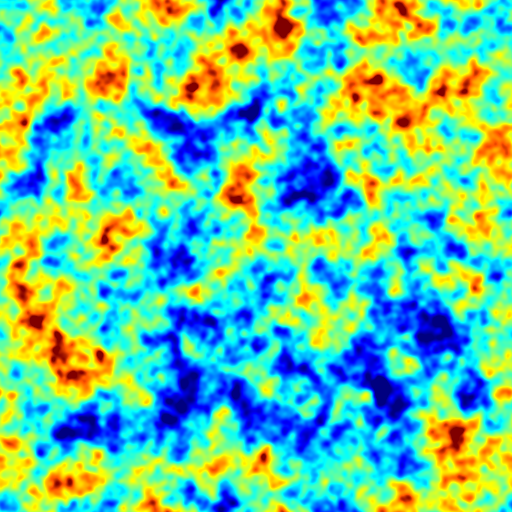
\includegraphics[height=7cm]{lensing/T.png}};}%
			\only<3>{\node at (0,0) {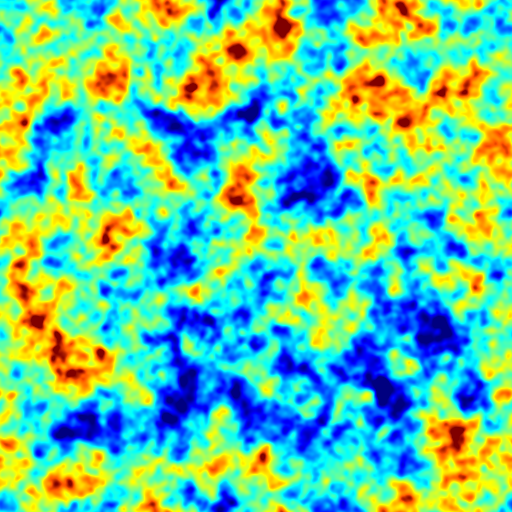
\includegraphics[height=7cm]{lensing/TlT.png}};}%
			\only<4-5>{\node at (0,0) {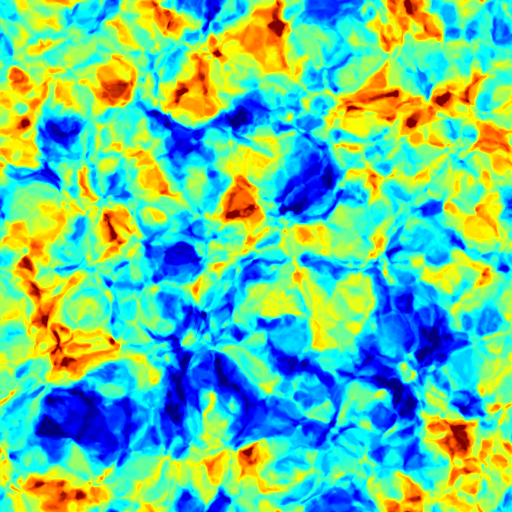
\includegraphics[height=7cm]{lensing/TsT.png}};}%
			\only<2-4>{\node at (0,0) {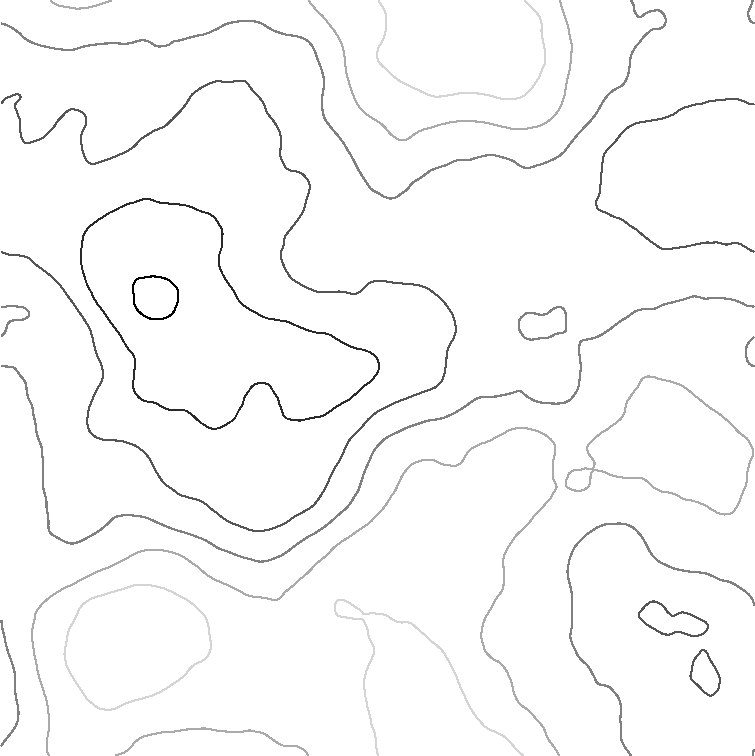
\includegraphics[height=7cm]{lensing/phi_contours.png}};}%
		\end{tikzpicture}

		\only<1>{Unlensed\uncover<0>{p}}%
		\only<2>{Gravitational potential}%
		\only<3>{Lensed\uncover<0>{p}}%
		\only<4>{Lensed x10\uncover<0>{p}}%
		\only<5>{Non-Gaussian\uncover<0>{p}}%
	\end{center}
\end{frame}

\begin{frame}{Lensing distorts the CMB Polarization}
	\begin{center}
		\hspace*{-3mm}
		\begin{tabular}{cc}
			{\bf Q} ($\pm 20\mu$K) & {\bf U} ($\pm 20\mu$K) \\
			\only<1>{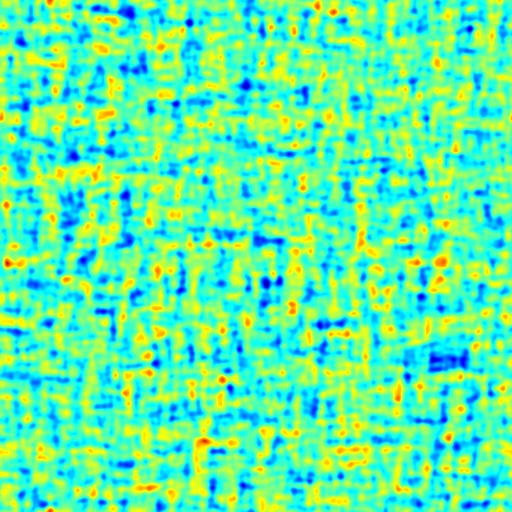
\includegraphics[height=5.5cm]{lensing/EBQ.png}}%
			\only<2>{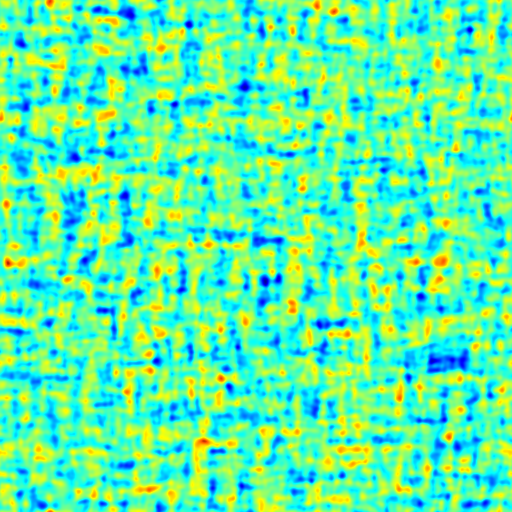
\includegraphics[height=5.5cm]{lensing/EBlQ.png}}%
			&
			\only<1>{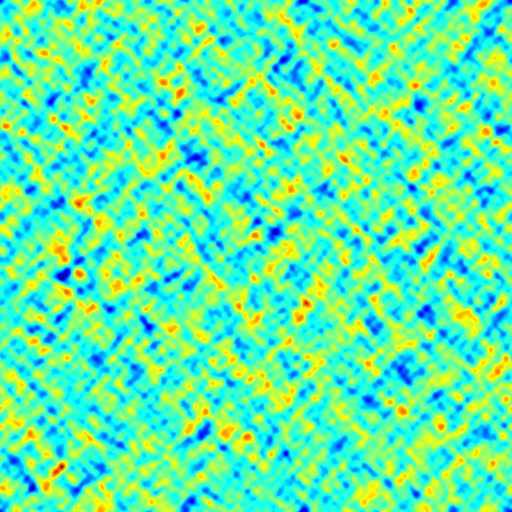
\includegraphics[height=5.5cm]{lensing/EBU.png}}%
			\only<2>{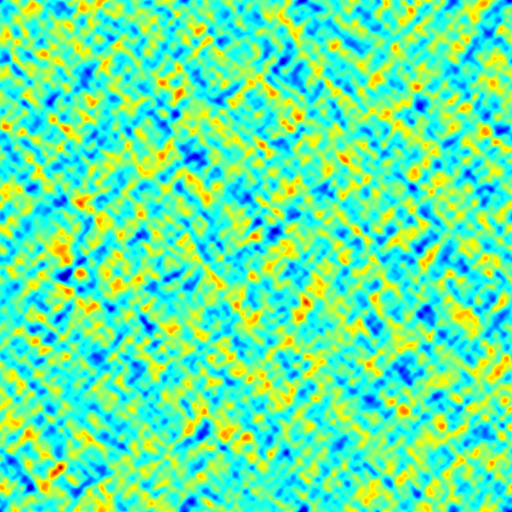
\includegraphics[height=5.5cm]{lensing/EBlU.png}}%
		\end{tabular}

		\only<1>{Unlensed}%
		\only<2>{Lensed}%
	\end{center}
\end{frame}

\begin{frame}{Lensing distorts E and B}
	\begin{center}
		\hspace*{-3mm}
		\begin{tabular}{cc}
			{\bf E} ($\pm 20\mu$K) & {\bf B} ($\pm 0.5\mu$K) \\
			\only<1>{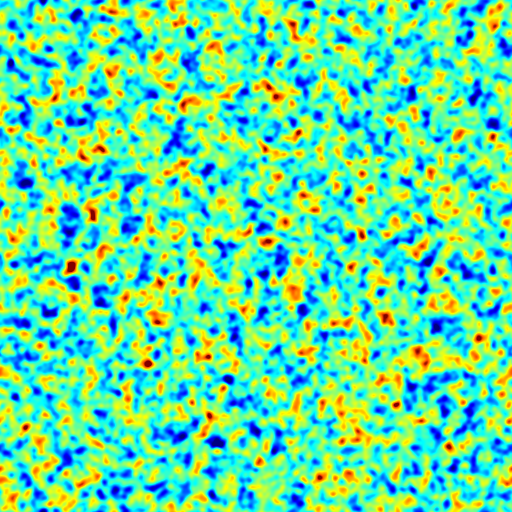
\includegraphics[height=5.5cm]{lensing/E.png}}%
			\only<2>{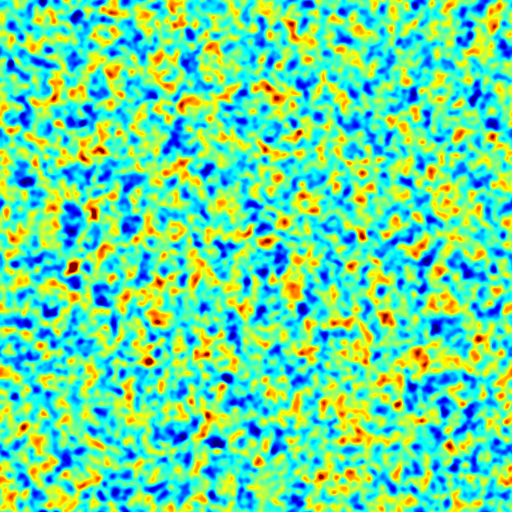
\includegraphics[height=5.5cm]{lensing/EBlE.png}}%
			&
			\only<1>{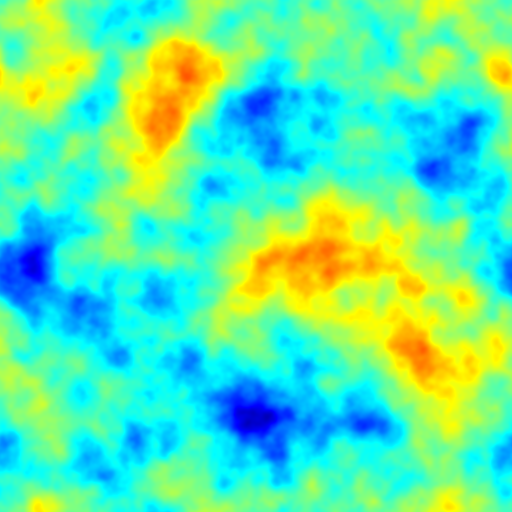
\includegraphics[height=5.5cm]{lensing/B.png}}%
			\only<2>{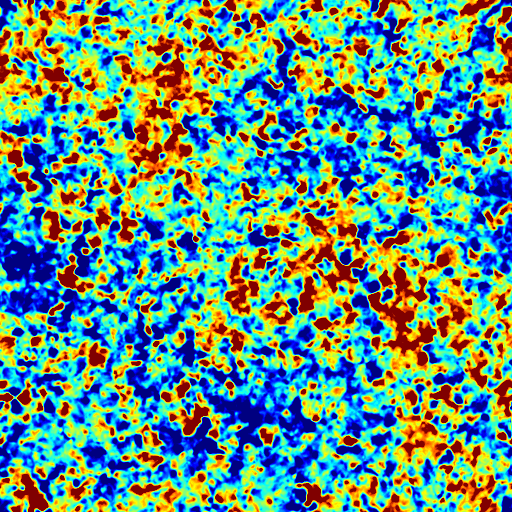
\includegraphics[height=5.5cm]{lensing/EBlB.png}}%
		\end{tabular}

		\only<1>{Unlensed}%
		\only<2>{Lensed}%
	\end{center}
\end{frame}

\end{document}
